\documentclass[twoside]{book}

% Packages required by doxygen
\usepackage{calc}
\usepackage{doxygen}
\usepackage{graphicx}
\usepackage[utf8]{inputenc}
\usepackage{makeidx}
\usepackage{multicol}
\usepackage{multirow}
\usepackage{textcomp}
\usepackage[table]{xcolor}

% Font selection
\usepackage[T1]{fontenc}
\usepackage{mathptmx}
\usepackage[scaled=.90]{helvet}
\usepackage{courier}
\usepackage{amssymb}
\usepackage{sectsty}
\renewcommand{\familydefault}{\sfdefault}
\allsectionsfont{%
  \fontseries{bc}\selectfont%
  \color{darkgray}%
}
\renewcommand{\DoxyLabelFont}{%
  \fontseries{bc}\selectfont%
  \color{darkgray}%
}

% Page & text layout
\usepackage{geometry}
\geometry{%
  a4paper,%
  top=2.5cm,%
  bottom=2.5cm,%
  left=2.5cm,%
  right=2.5cm%
}
\tolerance=750
\hfuzz=15pt
\hbadness=750
\setlength{\emergencystretch}{15pt}
\setlength{\parindent}{0cm}
\setlength{\parskip}{0.2cm}
\makeatletter
\renewcommand{\paragraph}{%
  \@startsection{paragraph}{4}{0ex}{-1.0ex}{1.0ex}{%
    \normalfont\normalsize\bfseries\SS@parafont%
  }%
}
\renewcommand{\subparagraph}{%
  \@startsection{subparagraph}{5}{0ex}{-1.0ex}{1.0ex}{%
    \normalfont\normalsize\bfseries\SS@subparafont%
  }%
}
\makeatother

% Headers & footers
\usepackage{fancyhdr}
\pagestyle{fancyplain}
\fancyhead[LE]{\fancyplain{}{\bfseries\thepage}}
\fancyhead[CE]{\fancyplain{}{}}
\fancyhead[RE]{\fancyplain{}{\bfseries\leftmark}}
\fancyhead[LO]{\fancyplain{}{\bfseries\rightmark}}
\fancyhead[CO]{\fancyplain{}{}}
\fancyhead[RO]{\fancyplain{}{\bfseries\thepage}}
\fancyfoot[LE]{\fancyplain{}{}}
\fancyfoot[CE]{\fancyplain{}{}}
\fancyfoot[RE]{\fancyplain{}{\bfseries\scriptsize Generated on Fri Jun 21 2013 14:44:57 for sourceBox by Doxygen }}
\fancyfoot[LO]{\fancyplain{}{\bfseries\scriptsize Generated on Fri Jun 21 2013 14:44:57 for sourceBox by Doxygen }}
\fancyfoot[CO]{\fancyplain{}{}}
\fancyfoot[RO]{\fancyplain{}{}}
\renewcommand{\footrulewidth}{0.4pt}
\renewcommand{\chaptermark}[1]{%
  \markboth{#1}{}%
}
\renewcommand{\sectionmark}[1]{%
  \markright{\thesection\ #1}%
}

% Indices & bibliography
\usepackage{natbib}
\usepackage[titles]{tocloft}
\setcounter{tocdepth}{3}
\setcounter{secnumdepth}{5}
\makeindex

% Hyperlinks (required, but should be loaded last)
\usepackage{ifpdf}
\ifpdf
  \usepackage[pdftex,pagebackref=true]{hyperref}
\else
  \usepackage[ps2pdf,pagebackref=true]{hyperref}
\fi
\hypersetup{%
  colorlinks=true,%
  linkcolor=blue,%
  citecolor=blue,%
  unicode%
}

% Custom commands
\newcommand{\clearemptydoublepage}{%
  \newpage{\pagestyle{empty}\cleardoublepage}%
}


%===== C O N T E N T S =====

\begin{document}

% Titlepage & ToC
\hypersetup{pageanchor=false}
\pagenumbering{roman}
\begin{titlepage}
\vspace*{7cm}
\begin{center}%
{\Large source\-Box \\[1ex]\large 1.\-0 }\\
\vspace*{1cm}
{\large Generated by Doxygen 1.8.4}\\
\vspace*{0.5cm}
{\small Fri Jun 21 2013 14:44:57}\\
\end{center}
\end{titlepage}
\clearemptydoublepage
\tableofcontents
\clearemptydoublepage
\pagenumbering{arabic}
\hypersetup{pageanchor=true}

%--- Begin generated contents ---
\chapter{Namespace Index}
\section{Namespace List}
Here is a list of all documented namespaces with brief descriptions\-:\begin{DoxyCompactList}
\item\contentsline{section}{\hyperlink{namespace_data___controller}{Data\-\_\-\-Controller} \\*Handles the communication with the backend }{\pageref{namespace_data___controller}}{}
\item\contentsline{section}{\hyperlink{namespacesrc_1_1communication__controller}{src.\-communication\-\_\-controller} }{\pageref{namespacesrc_1_1communication__controller}}{}
\item\contentsline{section}{\hyperlink{namespacesrc_1_1rcslib}{src.\-rcslib} }{\pageref{namespacesrc_1_1rcslib}}{}
\end{DoxyCompactList}

\chapter{Hierarchical Index}
\section{Class Hierarchy}
This inheritance list is sorted roughly, but not completely, alphabetically\-:\begin{DoxyCompactList}
\item object\begin{DoxyCompactList}
\item \contentsline{section}{src.\-\_\-\-\_\-main\-\_\-\-\_\-.\-Source\-Box\-Server}{\pageref{classsrc_1_1____main_____1_1_source_box_server}}{}
\item \contentsline{section}{src.\-communication\-\_\-controller.\-Communication\-\_\-\-Controller}{\pageref{classsrc_1_1communication__controller_1_1_communication___controller}}{}
\item \contentsline{section}{src.\-communication\-\_\-controller.\-Communication\-\_\-\-Controller}{\pageref{classsrc_1_1communication__controller_1_1_communication___controller}}{}
\item \contentsline{section}{src.\-data\-\_\-controller.\-Data\-\_\-\-Controller}{\pageref{classsrc_1_1data__controller_1_1_data___controller}}{}
\item \contentsline{section}{src.\-watchdog.\-Filesystem\-\_\-\-Controller}{\pageref{classsrc_1_1watchdog_1_1_filesystem___controller}}{}
\end{DoxyCompactList}
\item \contentsline{section}{src.\-rcslib.\-R\-C\-S}{\pageref{classsrc_1_1rcslib_1_1_r_c_s}}{}
\item File\-System\-Event\-Handler\begin{DoxyCompactList}
\item \contentsline{section}{src.\-\_\-\-\_\-main\-\_\-\-\_\-.\-My\-Event\-Handler}{\pageref{classsrc_1_1____main_____1_1_my_event_handler}}{}
\end{DoxyCompactList}
\end{DoxyCompactList}

\chapter{Class Index}
\section{Class List}
Here are the classes, structs, unions and interfaces with brief descriptions\-:\begin{DoxyCompactList}
\item\contentsline{section}{\hyperlink{classsrc_1_1communication__controller_1_1_communication___controller}{src.\-communication\-\_\-controller.\-Communication\-\_\-\-Controller} }{\pageref{classsrc_1_1communication__controller_1_1_communication___controller}}{}
\item\contentsline{section}{\hyperlink{classsrc_1_1data__controller_1_1_data___controller}{src.\-data\-\_\-controller.\-Data\-\_\-\-Controller} }{\pageref{classsrc_1_1data__controller_1_1_data___controller}}{}
\item\contentsline{section}{\hyperlink{classsrc_1_1watchdog_1_1_filesystem___controller}{src.\-watchdog.\-Filesystem\-\_\-\-Controller} }{\pageref{classsrc_1_1watchdog_1_1_filesystem___controller}}{}
\item\contentsline{section}{\hyperlink{classsrc_1_1____main_____1_1_my_event_handler}{src.\-\_\-\-\_\-main\-\_\-\-\_\-.\-My\-Event\-Handler} \\*

 \subsubsection*{C\-R\-E\-A\-T\-E F\-I\-L\-E\-S\-Y\-S\-T\-E\-M E\-V\-E\-N\-T H\-A\-N\-D\-L\-E\-R }}{\pageref{classsrc_1_1____main_____1_1_my_event_handler}}{}
\item\contentsline{section}{\hyperlink{classsrc_1_1rcslib_1_1_r_c_s}{src.\-rcslib.\-R\-C\-S} }{\pageref{classsrc_1_1rcslib_1_1_r_c_s}}{}
\item\contentsline{section}{\hyperlink{classsrc_1_1____main_____1_1_source_box_server}{src.\-\_\-\-\_\-main\-\_\-\-\_\-.\-Source\-Box\-Server} }{\pageref{classsrc_1_1____main_____1_1_source_box_server}}{}
\end{DoxyCompactList}

\chapter{Namespace Documentation}
\hypertarget{namespace_data___controller}{\section{Data\-\_\-\-Controller Namespace Reference}
\label{namespace_data___controller}\index{Data\-\_\-\-Controller@{Data\-\_\-\-Controller}}
}


handles the communication with the backend  




\subsection{Detailed Description}
handles the communication with the backend U\-T\-F-\/8, tabwidth = , newline = L\-F \begin{DoxyAuthor}{Author}
Martin 
\end{DoxyAuthor}

\hypertarget{namespacesrc_1_1communication__controller}{\section{src.\-communication\-\_\-controller Namespace Reference}
\label{namespacesrc_1_1communication__controller}\index{src.\-communication\-\_\-controller@{src.\-communication\-\_\-controller}}
}
\subsection*{Classes}
\begin{DoxyCompactItemize}
\item 
class \hyperlink{classsrc_1_1communication__controller_1_1_communication___controller}{Communication\-\_\-\-Controller}
\end{DoxyCompactItemize}


\subsection{Detailed Description}
\begin{DoxyVerb}-------------------------------------------------------------
' sourceboxclient – communication_controller
' handles the communication with the server
'
' @encode:  UTF-8, tabwidth = , newline = LF
' @date:    03.06.13
' @author:  GRUPPE 4 – Emanuel, wer noch?
'
'----------------------------------------------------------- \end{DoxyVerb}
 
\hypertarget{namespacesrc_1_1rcslib}{\section{src.\-rcslib Namespace Reference}
\label{namespacesrc_1_1rcslib}\index{src.\-rcslib@{src.\-rcslib}}
}
\subsection*{Classes}
\begin{DoxyCompactItemize}
\item 
class \hyperlink{classsrc_1_1rcslib_1_1_r_c_s}{R\-C\-S}
\end{DoxyCompactItemize}


\subsection{Detailed Description}
\begin{DoxyVerb}RCS interface module.

Defines the class RCS, which represents a directory with rcs version
files and (possibly) corresponding work files.\end{DoxyVerb}
 
\chapter{Class Documentation}
\hypertarget{classsrc_1_1communication__controller_1_1_communication___controller}{\section{src.\-communication\-\_\-controller.\-Communication\-\_\-\-Controller Class Reference}
\label{classsrc_1_1communication__controller_1_1_communication___controller}\index{src.\-communication\-\_\-controller.\-Communication\-\_\-\-Controller@{src.\-communication\-\_\-controller.\-Communication\-\_\-\-Controller}}
}
Inheritance diagram for src.\-communication\-\_\-controller.\-Communication\-\_\-\-Controller\-:\begin{figure}[H]
\begin{center}
\leavevmode
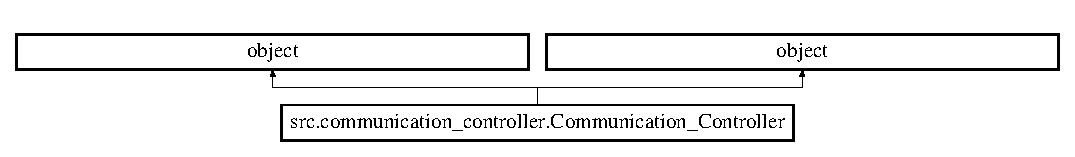
\includegraphics[height=1.656805cm]{classsrc_1_1communication__controller_1_1_communication___controller}
\end{center}
\end{figure}
\subsection*{Public Member Functions}
\begin{DoxyCompactItemize}
\item 
\hypertarget{classsrc_1_1communication__controller_1_1_communication___controller_a94862bb57729b432b60a8410290a3bf8}{def {\bfseries \-\_\-\-\_\-init\-\_\-\-\_\-}}\label{classsrc_1_1communication__controller_1_1_communication___controller_a94862bb57729b432b60a8410290a3bf8}

\item 
\hypertarget{classsrc_1_1communication__controller_1_1_communication___controller_aec0c66fcdd1004d21a80534d290e0a8e}{def {\bfseries update\-\_\-files}}\label{classsrc_1_1communication__controller_1_1_communication___controller_aec0c66fcdd1004d21a80534d290e0a8e}

\item 
\hypertarget{classsrc_1_1communication__controller_1_1_communication___controller_a4b5613ea0c4987288e539ed90c9af582}{def {\bfseries create\-\_\-file}}\label{classsrc_1_1communication__controller_1_1_communication___controller_a4b5613ea0c4987288e539ed90c9af582}

\item 
\hypertarget{classsrc_1_1communication__controller_1_1_communication___controller_a47092ca1a4a65b6363b6762087346074}{def {\bfseries lock\-\_\-file}}\label{classsrc_1_1communication__controller_1_1_communication___controller_a47092ca1a4a65b6363b6762087346074}

\item 
\hypertarget{classsrc_1_1communication__controller_1_1_communication___controller_a544c46299932b770685575cf7195db00}{def {\bfseries modify\-\_\-file}}\label{classsrc_1_1communication__controller_1_1_communication___controller_a544c46299932b770685575cf7195db00}

\item 
\hypertarget{classsrc_1_1communication__controller_1_1_communication___controller_ae41fb68815ce4c9fce84ec4d22baf1e9}{def {\bfseries unlock\-\_\-file}}\label{classsrc_1_1communication__controller_1_1_communication___controller_ae41fb68815ce4c9fce84ec4d22baf1e9}

\item 
\hypertarget{classsrc_1_1communication__controller_1_1_communication___controller_a72e1c71e0cb75efefa844e3a8eafc21c}{def {\bfseries delete\-\_\-file}}\label{classsrc_1_1communication__controller_1_1_communication___controller_a72e1c71e0cb75efefa844e3a8eafc21c}

\item 
\hypertarget{classsrc_1_1communication__controller_1_1_communication___controller_a94862bb57729b432b60a8410290a3bf8}{def {\bfseries \-\_\-\-\_\-init\-\_\-\-\_\-}}\label{classsrc_1_1communication__controller_1_1_communication___controller_a94862bb57729b432b60a8410290a3bf8}

\item 
\hypertarget{classsrc_1_1communication__controller_1_1_communication___controller_aec0c66fcdd1004d21a80534d290e0a8e}{def {\bfseries update\-\_\-files}}\label{classsrc_1_1communication__controller_1_1_communication___controller_aec0c66fcdd1004d21a80534d290e0a8e}

\item 
\hypertarget{classsrc_1_1communication__controller_1_1_communication___controller_a4b5613ea0c4987288e539ed90c9af582}{def {\bfseries create\-\_\-file}}\label{classsrc_1_1communication__controller_1_1_communication___controller_a4b5613ea0c4987288e539ed90c9af582}

\item 
\hypertarget{classsrc_1_1communication__controller_1_1_communication___controller_a47092ca1a4a65b6363b6762087346074}{def {\bfseries lock\-\_\-file}}\label{classsrc_1_1communication__controller_1_1_communication___controller_a47092ca1a4a65b6363b6762087346074}

\item 
\hypertarget{classsrc_1_1communication__controller_1_1_communication___controller_a544c46299932b770685575cf7195db00}{def {\bfseries modify\-\_\-file}}\label{classsrc_1_1communication__controller_1_1_communication___controller_a544c46299932b770685575cf7195db00}

\item 
\hypertarget{classsrc_1_1communication__controller_1_1_communication___controller_ae41fb68815ce4c9fce84ec4d22baf1e9}{def {\bfseries unlock\-\_\-file}}\label{classsrc_1_1communication__controller_1_1_communication___controller_ae41fb68815ce4c9fce84ec4d22baf1e9}

\item 
\hypertarget{classsrc_1_1communication__controller_1_1_communication___controller_a72e1c71e0cb75efefa844e3a8eafc21c}{def {\bfseries delete\-\_\-file}}\label{classsrc_1_1communication__controller_1_1_communication___controller_a72e1c71e0cb75efefa844e3a8eafc21c}

\end{DoxyCompactItemize}


The documentation for this class was generated from the following files\-:\begin{DoxyCompactItemize}
\item 
sourcebox-\/client/src/communication\-\_\-controller.\-py\item 
sourcebox-\/server/src/communication\-\_\-controller.\-py\end{DoxyCompactItemize}

\hypertarget{classsrc_1_1data__controller_1_1_data___controller}{\section{src.\-data\-\_\-controller.\-Data\-\_\-\-Controller Class Reference}
\label{classsrc_1_1data__controller_1_1_data___controller}\index{src.\-data\-\_\-controller.\-Data\-\_\-\-Controller@{src.\-data\-\_\-controller.\-Data\-\_\-\-Controller}}
}
Inheritance diagram for src.\-data\-\_\-controller.\-Data\-\_\-\-Controller\-:\begin{figure}[H]
\begin{center}
\leavevmode
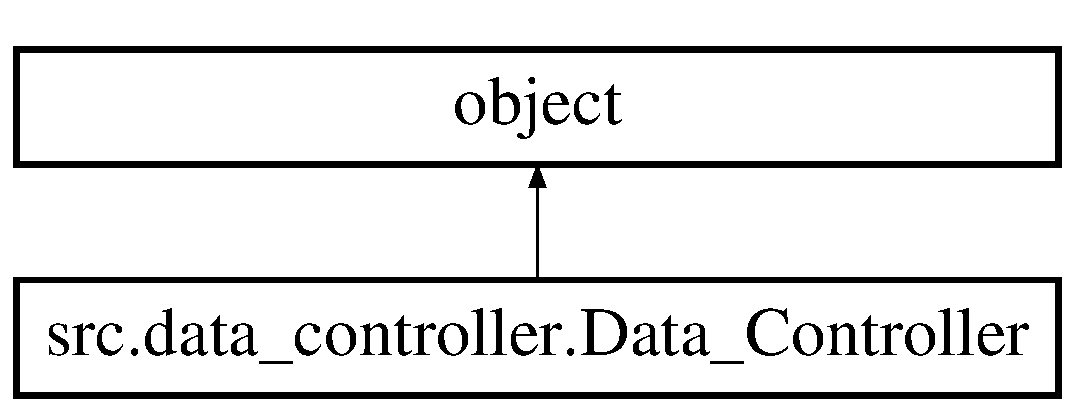
\includegraphics[height=2.000000cm]{classsrc_1_1data__controller_1_1_data___controller}
\end{center}
\end{figure}
\subsection*{Public Member Functions}
\begin{DoxyCompactItemize}
\item 
def \hyperlink{classsrc_1_1data__controller_1_1_data___controller_aebfcfd29fcba061bc85a646d6f0d6f7d}{\-\_\-\-\_\-init\-\_\-\-\_\-}
\begin{DoxyCompactList}\small\item\em Creates a new instance of the data controller. \end{DoxyCompactList}\item 
def \hyperlink{classsrc_1_1data__controller_1_1_data___controller_adbcacdf18408e165f067038d192d4d80}{read\-\_\-file}
\begin{DoxyCompactList}\small\item\em Reads a file. \end{DoxyCompactList}\item 
def \hyperlink{classsrc_1_1data__controller_1_1_data___controller_a279f3502ecae82adaa7c325abc2f2a5b}{is\-\_\-locked}
\begin{DoxyCompactList}\small\item\em Checks if a file is locked. \end{DoxyCompactList}\item 
def \hyperlink{classsrc_1_1data__controller_1_1_data___controller_a659bef775a5aabe125f808e05415bcf0}{lock\-\_\-file}
\begin{DoxyCompactList}\small\item\em Locks a file. \end{DoxyCompactList}\item 
def \hyperlink{classsrc_1_1data__controller_1_1_data___controller_a85947b341a0886aa2616a577b9876099}{unlock\-\_\-file}
\begin{DoxyCompactList}\small\item\em Unlocks a file. \end{DoxyCompactList}\item 
def \hyperlink{classsrc_1_1data__controller_1_1_data___controller_a47dac6b2ccb5cf3798e80c44a8c3b4cd}{delete\-\_\-file}
\begin{DoxyCompactList}\small\item\em Deletes a file. \end{DoxyCompactList}\item 
def \hyperlink{classsrc_1_1data__controller_1_1_data___controller_ad96deef27f2db007790c35c969ffaab9}{create\-\_\-file}
\begin{DoxyCompactList}\small\item\em Creates a new file. \end{DoxyCompactList}\item 
def \hyperlink{classsrc_1_1data__controller_1_1_data___controller_a7e0468161553dfb087390c3d289ad1fb}{save\-\_\-file}
\begin{DoxyCompactList}\small\item\em Saves a file. \end{DoxyCompactList}\item 
def \hyperlink{classsrc_1_1data__controller_1_1_data___controller_afa65bc68b8aba942e39ca55fc54c9345}{show\-\_\-changes}
\begin{DoxyCompactList}\small\item\em Show changes of the file. \end{DoxyCompactList}\end{DoxyCompactItemize}
\subsection*{Public Attributes}
\begin{DoxyCompactItemize}
\item 
\hypertarget{classsrc_1_1data__controller_1_1_data___controller_a75b9c57761e02379b5aa34921a41ee64}{{\bfseries rcs}}\label{classsrc_1_1data__controller_1_1_data___controller_a75b9c57761e02379b5aa34921a41ee64}

\end{DoxyCompactItemize}
\subsection*{Static Public Attributes}
\begin{DoxyCompactItemize}
\item 
\hypertarget{classsrc_1_1data__controller_1_1_data___controller_a28cc2edb8c605ddddfed48f1d89bff22}{string {\bfseries data\-\_\-dir} = ''}\label{classsrc_1_1data__controller_1_1_data___controller_a28cc2edb8c605ddddfed48f1d89bff22}

\end{DoxyCompactItemize}


\subsection{Constructor \& Destructor Documentation}
\hypertarget{classsrc_1_1data__controller_1_1_data___controller_aebfcfd29fcba061bc85a646d6f0d6f7d}{\index{src\-::data\-\_\-controller\-::\-Data\-\_\-\-Controller@{src\-::data\-\_\-controller\-::\-Data\-\_\-\-Controller}!\-\_\-\-\_\-init\-\_\-\-\_\-@{\-\_\-\-\_\-init\-\_\-\-\_\-}}
\index{\-\_\-\-\_\-init\-\_\-\-\_\-@{\-\_\-\-\_\-init\-\_\-\-\_\-}!src::data_controller::Data_Controller@{src\-::data\-\_\-controller\-::\-Data\-\_\-\-Controller}}
\subsubsection[{\-\_\-\-\_\-init\-\_\-\-\_\-}]{\setlength{\rightskip}{0pt plus 5cm}def src.\-data\-\_\-controller.\-Data\-\_\-\-Controller.\-\_\-\-\_\-init\-\_\-\-\_\- (
\begin{DoxyParamCaption}
\item[{}]{self, }
\item[{}]{data\-\_\-dir}
\end{DoxyParamCaption}
)}}\label{classsrc_1_1data__controller_1_1_data___controller_aebfcfd29fcba061bc85a646d6f0d6f7d}


Creates a new instance of the data controller. 


\begin{DoxyParams}{Parameters}
{\em data\-\_\-dir} & The directory where the data is being stored \\
\hline
\end{DoxyParams}


\subsection{Member Function Documentation}
\hypertarget{classsrc_1_1data__controller_1_1_data___controller_ad96deef27f2db007790c35c969ffaab9}{\index{src\-::data\-\_\-controller\-::\-Data\-\_\-\-Controller@{src\-::data\-\_\-controller\-::\-Data\-\_\-\-Controller}!create\-\_\-file@{create\-\_\-file}}
\index{create\-\_\-file@{create\-\_\-file}!src::data_controller::Data_Controller@{src\-::data\-\_\-controller\-::\-Data\-\_\-\-Controller}}
\subsubsection[{create\-\_\-file}]{\setlength{\rightskip}{0pt plus 5cm}def src.\-data\-\_\-controller.\-Data\-\_\-\-Controller.\-create\-\_\-file (
\begin{DoxyParamCaption}
\item[{}]{self, }
\item[{}]{file\-\_\-name}
\end{DoxyParamCaption}
)}}\label{classsrc_1_1data__controller_1_1_data___controller_ad96deef27f2db007790c35c969ffaab9}


Creates a new file. 


\begin{DoxyParams}{Parameters}
{\em file\-\_\-name} & name of the file \\
\hline
\end{DoxyParams}
\hypertarget{classsrc_1_1data__controller_1_1_data___controller_a47dac6b2ccb5cf3798e80c44a8c3b4cd}{\index{src\-::data\-\_\-controller\-::\-Data\-\_\-\-Controller@{src\-::data\-\_\-controller\-::\-Data\-\_\-\-Controller}!delete\-\_\-file@{delete\-\_\-file}}
\index{delete\-\_\-file@{delete\-\_\-file}!src::data_controller::Data_Controller@{src\-::data\-\_\-controller\-::\-Data\-\_\-\-Controller}}
\subsubsection[{delete\-\_\-file}]{\setlength{\rightskip}{0pt plus 5cm}def src.\-data\-\_\-controller.\-Data\-\_\-\-Controller.\-delete\-\_\-file (
\begin{DoxyParamCaption}
\item[{}]{self, }
\item[{}]{file\-\_\-name}
\end{DoxyParamCaption}
)}}\label{classsrc_1_1data__controller_1_1_data___controller_a47dac6b2ccb5cf3798e80c44a8c3b4cd}


Deletes a file. 


\begin{DoxyParams}{Parameters}
{\em file\-\_\-name} & name of the file \\
\hline
\end{DoxyParams}
\hypertarget{classsrc_1_1data__controller_1_1_data___controller_a279f3502ecae82adaa7c325abc2f2a5b}{\index{src\-::data\-\_\-controller\-::\-Data\-\_\-\-Controller@{src\-::data\-\_\-controller\-::\-Data\-\_\-\-Controller}!is\-\_\-locked@{is\-\_\-locked}}
\index{is\-\_\-locked@{is\-\_\-locked}!src::data_controller::Data_Controller@{src\-::data\-\_\-controller\-::\-Data\-\_\-\-Controller}}
\subsubsection[{is\-\_\-locked}]{\setlength{\rightskip}{0pt plus 5cm}def src.\-data\-\_\-controller.\-Data\-\_\-\-Controller.\-is\-\_\-locked (
\begin{DoxyParamCaption}
\item[{}]{self, }
\item[{}]{file\-\_\-name}
\end{DoxyParamCaption}
)}}\label{classsrc_1_1data__controller_1_1_data___controller_a279f3502ecae82adaa7c325abc2f2a5b}


Checks if a file is locked. 


\begin{DoxyParams}{Parameters}
{\em file\-\_\-name} & name of the file \\
\hline
\end{DoxyParams}
\hypertarget{classsrc_1_1data__controller_1_1_data___controller_a659bef775a5aabe125f808e05415bcf0}{\index{src\-::data\-\_\-controller\-::\-Data\-\_\-\-Controller@{src\-::data\-\_\-controller\-::\-Data\-\_\-\-Controller}!lock\-\_\-file@{lock\-\_\-file}}
\index{lock\-\_\-file@{lock\-\_\-file}!src::data_controller::Data_Controller@{src\-::data\-\_\-controller\-::\-Data\-\_\-\-Controller}}
\subsubsection[{lock\-\_\-file}]{\setlength{\rightskip}{0pt plus 5cm}def src.\-data\-\_\-controller.\-Data\-\_\-\-Controller.\-lock\-\_\-file (
\begin{DoxyParamCaption}
\item[{}]{self, }
\item[{}]{file\-\_\-name}
\end{DoxyParamCaption}
)}}\label{classsrc_1_1data__controller_1_1_data___controller_a659bef775a5aabe125f808e05415bcf0}


Locks a file. 


\begin{DoxyParams}{Parameters}
{\em file\-\_\-name} & name of the file \\
\hline
\end{DoxyParams}
\hypertarget{classsrc_1_1data__controller_1_1_data___controller_adbcacdf18408e165f067038d192d4d80}{\index{src\-::data\-\_\-controller\-::\-Data\-\_\-\-Controller@{src\-::data\-\_\-controller\-::\-Data\-\_\-\-Controller}!read\-\_\-file@{read\-\_\-file}}
\index{read\-\_\-file@{read\-\_\-file}!src::data_controller::Data_Controller@{src\-::data\-\_\-controller\-::\-Data\-\_\-\-Controller}}
\subsubsection[{read\-\_\-file}]{\setlength{\rightskip}{0pt plus 5cm}def src.\-data\-\_\-controller.\-Data\-\_\-\-Controller.\-read\-\_\-file (
\begin{DoxyParamCaption}
\item[{}]{self, }
\item[{}]{file\-\_\-name}
\end{DoxyParamCaption}
)}}\label{classsrc_1_1data__controller_1_1_data___controller_adbcacdf18408e165f067038d192d4d80}


Reads a file. 


\begin{DoxyParams}{Parameters}
{\em file\-\_\-name} & name of the file \\
\hline
\end{DoxyParams}
\hypertarget{classsrc_1_1data__controller_1_1_data___controller_a7e0468161553dfb087390c3d289ad1fb}{\index{src\-::data\-\_\-controller\-::\-Data\-\_\-\-Controller@{src\-::data\-\_\-controller\-::\-Data\-\_\-\-Controller}!save\-\_\-file@{save\-\_\-file}}
\index{save\-\_\-file@{save\-\_\-file}!src::data_controller::Data_Controller@{src\-::data\-\_\-controller\-::\-Data\-\_\-\-Controller}}
\subsubsection[{save\-\_\-file}]{\setlength{\rightskip}{0pt plus 5cm}def src.\-data\-\_\-controller.\-Data\-\_\-\-Controller.\-save\-\_\-file (
\begin{DoxyParamCaption}
\item[{}]{self, }
\item[{}]{file\-\_\-name, }
\item[{}]{content}
\end{DoxyParamCaption}
)}}\label{classsrc_1_1data__controller_1_1_data___controller_a7e0468161553dfb087390c3d289ad1fb}


Saves a file. 


\begin{DoxyParams}{Parameters}
{\em file\-\_\-name} & name of the file \\
\hline
{\em content} & the content to be stored in the file \\
\hline
\end{DoxyParams}
\hypertarget{classsrc_1_1data__controller_1_1_data___controller_afa65bc68b8aba942e39ca55fc54c9345}{\index{src\-::data\-\_\-controller\-::\-Data\-\_\-\-Controller@{src\-::data\-\_\-controller\-::\-Data\-\_\-\-Controller}!show\-\_\-changes@{show\-\_\-changes}}
\index{show\-\_\-changes@{show\-\_\-changes}!src::data_controller::Data_Controller@{src\-::data\-\_\-controller\-::\-Data\-\_\-\-Controller}}
\subsubsection[{show\-\_\-changes}]{\setlength{\rightskip}{0pt plus 5cm}def src.\-data\-\_\-controller.\-Data\-\_\-\-Controller.\-show\-\_\-changes (
\begin{DoxyParamCaption}
\item[{}]{self, }
\item[{}]{file\-\_\-name}
\end{DoxyParamCaption}
)}}\label{classsrc_1_1data__controller_1_1_data___controller_afa65bc68b8aba942e39ca55fc54c9345}


Show changes of the file. 


\begin{DoxyParams}{Parameters}
{\em file\-\_\-name} & name of the file \\
\hline
\end{DoxyParams}
\hypertarget{classsrc_1_1data__controller_1_1_data___controller_a85947b341a0886aa2616a577b9876099}{\index{src\-::data\-\_\-controller\-::\-Data\-\_\-\-Controller@{src\-::data\-\_\-controller\-::\-Data\-\_\-\-Controller}!unlock\-\_\-file@{unlock\-\_\-file}}
\index{unlock\-\_\-file@{unlock\-\_\-file}!src::data_controller::Data_Controller@{src\-::data\-\_\-controller\-::\-Data\-\_\-\-Controller}}
\subsubsection[{unlock\-\_\-file}]{\setlength{\rightskip}{0pt plus 5cm}def src.\-data\-\_\-controller.\-Data\-\_\-\-Controller.\-unlock\-\_\-file (
\begin{DoxyParamCaption}
\item[{}]{self, }
\item[{}]{file\-\_\-name}
\end{DoxyParamCaption}
)}}\label{classsrc_1_1data__controller_1_1_data___controller_a85947b341a0886aa2616a577b9876099}


Unlocks a file. 


\begin{DoxyParams}{Parameters}
{\em file\-\_\-name} & name of the file \\
\hline
\end{DoxyParams}


The documentation for this class was generated from the following file\-:\begin{DoxyCompactItemize}
\item 
sourcebox-\/server/src/data\-\_\-controller.\-py\end{DoxyCompactItemize}

\hypertarget{classsrc_1_1watchdog_1_1_filesystem___controller}{\section{src.\-watchdog.\-Filesystem\-\_\-\-Controller Class Reference}
\label{classsrc_1_1watchdog_1_1_filesystem___controller}\index{src.\-watchdog.\-Filesystem\-\_\-\-Controller@{src.\-watchdog.\-Filesystem\-\_\-\-Controller}}
}
Inheritance diagram for src.\-watchdog.\-Filesystem\-\_\-\-Controller\-:\begin{figure}[H]
\begin{center}
\leavevmode
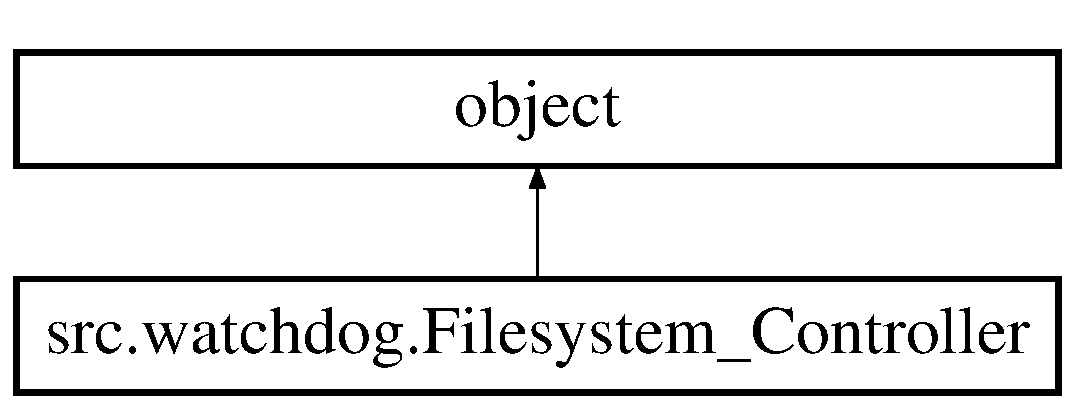
\includegraphics[height=2.000000cm]{classsrc_1_1watchdog_1_1_filesystem___controller}
\end{center}
\end{figure}
\subsection*{Public Member Functions}
\begin{DoxyCompactItemize}
\item 
\hypertarget{classsrc_1_1watchdog_1_1_filesystem___controller_a69037ccdf91029b3836e15808cb5eefd}{def {\bfseries \-\_\-\-\_\-init\-\_\-\-\_\-}}\label{classsrc_1_1watchdog_1_1_filesystem___controller_a69037ccdf91029b3836e15808cb5eefd}

\end{DoxyCompactItemize}


The documentation for this class was generated from the following file\-:\begin{DoxyCompactItemize}
\item 
sourcebox-\/client/src/watchdog.\-py\end{DoxyCompactItemize}

\hypertarget{classsrc_1_1____main_____1_1_my_event_handler}{\section{src.\-\_\-\-\_\-main\-\_\-\-\_\-.\-My\-Event\-Handler Class Reference}
\label{classsrc_1_1____main_____1_1_my_event_handler}\index{src.\-\_\-\-\_\-main\-\_\-\-\_\-.\-My\-Event\-Handler@{src.\-\_\-\-\_\-main\-\_\-\-\_\-.\-My\-Event\-Handler}}
}




 \subsubsection*{C\-R\-E\-A\-T\-E F\-I\-L\-E\-S\-Y\-S\-T\-E\-M E\-V\-E\-N\-T H\-A\-N\-D\-L\-E\-R } 


Inheritance diagram for src.\-\_\-\-\_\-main\-\_\-\-\_\-.\-My\-Event\-Handler\-:\begin{figure}[H]
\begin{center}
\leavevmode
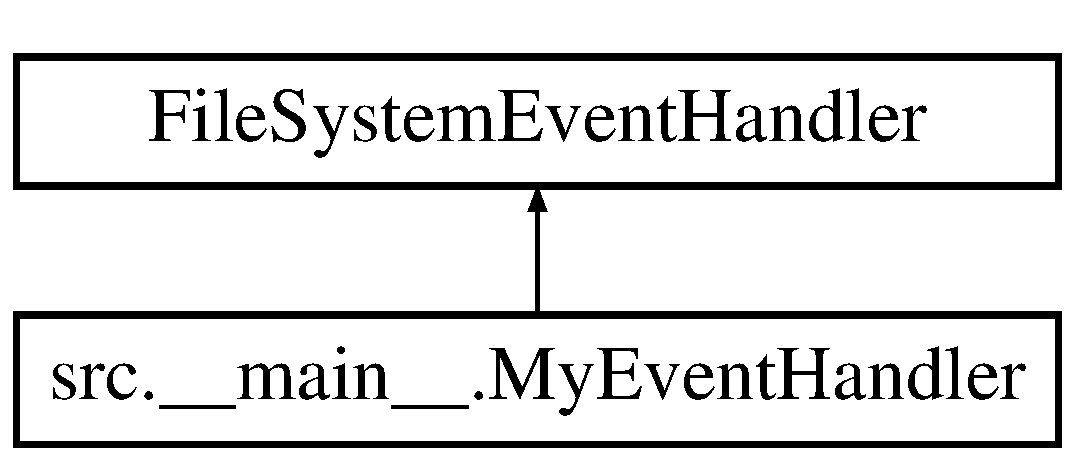
\includegraphics[height=2.000000cm]{classsrc_1_1____main_____1_1_my_event_handler}
\end{center}
\end{figure}
\subsection*{Public Member Functions}
\begin{DoxyCompactItemize}
\item 
\hypertarget{classsrc_1_1____main_____1_1_my_event_handler_a65873e108187474f10c5edc4cf58051d}{def {\bfseries \-\_\-\-\_\-init\-\_\-\-\_\-}}\label{classsrc_1_1____main_____1_1_my_event_handler_a65873e108187474f10c5edc4cf58051d}

\item 
\hypertarget{classsrc_1_1____main_____1_1_my_event_handler_a601600b8fc80783b92efb7729def7b99}{def {\bfseries on\-\_\-created}}\label{classsrc_1_1____main_____1_1_my_event_handler_a601600b8fc80783b92efb7729def7b99}

\item 
\hypertarget{classsrc_1_1____main_____1_1_my_event_handler_a87c6af0c4ed396bfd9f1532ee2e52fdd}{def {\bfseries on\-\_\-deleted}}\label{classsrc_1_1____main_____1_1_my_event_handler_a87c6af0c4ed396bfd9f1532ee2e52fdd}

\item 
\hypertarget{classsrc_1_1____main_____1_1_my_event_handler_add6f4372401415fe377688acf35fd6db}{def {\bfseries on\-\_\-modified}}\label{classsrc_1_1____main_____1_1_my_event_handler_add6f4372401415fe377688acf35fd6db}

\item 
\hypertarget{classsrc_1_1____main_____1_1_my_event_handler_ab6e207b1d506c9002f68076cc54710a3}{def {\bfseries on\-\_\-moved}}\label{classsrc_1_1____main_____1_1_my_event_handler_ab6e207b1d506c9002f68076cc54710a3}

\end{DoxyCompactItemize}
\subsection*{Public Attributes}
\begin{DoxyCompactItemize}
\item 
\hypertarget{classsrc_1_1____main_____1_1_my_event_handler_a499a542c02cff1006f2842b4c873ac7c}{{\bfseries observer}}\label{classsrc_1_1____main_____1_1_my_event_handler_a499a542c02cff1006f2842b4c873ac7c}

\end{DoxyCompactItemize}


\subsection{Detailed Description}


 \subsubsection*{C\-R\-E\-A\-T\-E F\-I\-L\-E\-S\-Y\-S\-T\-E\-M E\-V\-E\-N\-T H\-A\-N\-D\-L\-E\-R }

The documentation for this class was generated from the following file\-:\begin{DoxyCompactItemize}
\item 
sourcebox-\/client/src/\-\_\-\-\_\-main\-\_\-\-\_\-.\-py\end{DoxyCompactItemize}

\hypertarget{classsrc_1_1rcslib_1_1_r_c_s}{\section{src.\-rcslib.\-R\-C\-S Class Reference}
\label{classsrc_1_1rcslib_1_1_r_c_s}\index{src.\-rcslib.\-R\-C\-S@{src.\-rcslib.\-R\-C\-S}}
}
\subsection*{Public Member Functions}
\begin{DoxyCompactItemize}
\item 
def \hyperlink{classsrc_1_1rcslib_1_1_r_c_s_af6d3f83ff6e44adfd44ba8dae37e65c4}{\-\_\-\-\_\-init\-\_\-\-\_\-}
\item 
def \hyperlink{classsrc_1_1rcslib_1_1_r_c_s_a9bfcc8c2d943fa305ddc4f97cf54e6a9}{\-\_\-\-\_\-del\-\_\-\-\_\-}
\item 
def \hyperlink{classsrc_1_1rcslib_1_1_r_c_s_a907e8db00fe010cad8fa0f20173f9b9a}{log}
\item 
def \hyperlink{classsrc_1_1rcslib_1_1_r_c_s_a984a594621aacbf75eaab80bbbe61eb6}{head}
\item 
def \hyperlink{classsrc_1_1rcslib_1_1_r_c_s_a8e83cec89e260b48c055406b9345438a}{info}
\item 
def \hyperlink{classsrc_1_1rcslib_1_1_r_c_s_a70fe29b9b6df38d982c90c9f966db453}{lock}
\item 
def \hyperlink{classsrc_1_1rcslib_1_1_r_c_s_a5682c4e36636c6d5fa260c2fdc7b94a2}{unlock}
\item 
def \hyperlink{classsrc_1_1rcslib_1_1_r_c_s_a4d90840fd169eb50f41cb66acc6e672a}{checkout}
\item 
def \hyperlink{classsrc_1_1rcslib_1_1_r_c_s_ad3a4f70c5fbe84a0e42ca943428f55d2}{checkin}
\item 
def \hyperlink{classsrc_1_1rcslib_1_1_r_c_s_ad7ddfde96181fc65b61fa2cc8df7acb8}{listfiles}
\item 
def \hyperlink{classsrc_1_1rcslib_1_1_r_c_s_af22029df600c226a8462bc6228621265}{isvalid}
\item 
def \hyperlink{classsrc_1_1rcslib_1_1_r_c_s_a2c31aea9df8c203cf687cf8dbbb23075}{rcsname}
\item 
def \hyperlink{classsrc_1_1rcslib_1_1_r_c_s_a7fecb235e4ecd26ff89000fde665000e}{realname}
\item 
def \hyperlink{classsrc_1_1rcslib_1_1_r_c_s_a5f6f4c966126cb67ac9d82be61af3afc}{islocked}
\item 
def \hyperlink{classsrc_1_1rcslib_1_1_r_c_s_aba91cf3ead7caee48101e0fcd0af908b}{checkfile}
\end{DoxyCompactItemize}
\subsection*{Static Public Attributes}
\begin{DoxyCompactItemize}
\item 
\hypertarget{classsrc_1_1rcslib_1_1_r_c_s_ae1c303bd984c0c32e2bc6217ac1c21d8}{string {\bfseries okchars} = string.\-ascii\-\_\-letters+string.\-digits+'-\/\-\_\-=+'}\label{classsrc_1_1rcslib_1_1_r_c_s_ae1c303bd984c0c32e2bc6217ac1c21d8}

\end{DoxyCompactItemize}


\subsection{Detailed Description}
\begin{DoxyVerb}RCS interface class (local filesystem version).

An instance of this class represents a directory with rcs version
files and (possible) corresponding work files.

Methods provide access to most rcs operations such as
checkin/checkout, access to the rcs metadata (revisions, logs,
branches etc.) as well as some filesystem operations such as
listing all rcs version files.

XXX BUGS / PROBLEMS

- The instance always represents the current directory so it's not
very useful to have more than one instance around simultaneously\end{DoxyVerb}
 

\subsection{Constructor \& Destructor Documentation}
\hypertarget{classsrc_1_1rcslib_1_1_r_c_s_af6d3f83ff6e44adfd44ba8dae37e65c4}{\index{src\-::rcslib\-::\-R\-C\-S@{src\-::rcslib\-::\-R\-C\-S}!\-\_\-\-\_\-init\-\_\-\-\_\-@{\-\_\-\-\_\-init\-\_\-\-\_\-}}
\index{\-\_\-\-\_\-init\-\_\-\-\_\-@{\-\_\-\-\_\-init\-\_\-\-\_\-}!src::rcslib::RCS@{src\-::rcslib\-::\-R\-C\-S}}
\subsubsection[{\-\_\-\-\_\-init\-\_\-\-\_\-}]{\setlength{\rightskip}{0pt plus 5cm}def src.\-rcslib.\-R\-C\-S.\-\_\-\-\_\-init\-\_\-\-\_\- (
\begin{DoxyParamCaption}
\item[{}]{self}
\end{DoxyParamCaption}
)}}\label{classsrc_1_1rcslib_1_1_r_c_s_af6d3f83ff6e44adfd44ba8dae37e65c4}
\begin{DoxyVerb}Constructor.\end{DoxyVerb}
 \hypertarget{classsrc_1_1rcslib_1_1_r_c_s_a9bfcc8c2d943fa305ddc4f97cf54e6a9}{\index{src\-::rcslib\-::\-R\-C\-S@{src\-::rcslib\-::\-R\-C\-S}!\-\_\-\-\_\-del\-\_\-\-\_\-@{\-\_\-\-\_\-del\-\_\-\-\_\-}}
\index{\-\_\-\-\_\-del\-\_\-\-\_\-@{\-\_\-\-\_\-del\-\_\-\-\_\-}!src::rcslib::RCS@{src\-::rcslib\-::\-R\-C\-S}}
\subsubsection[{\-\_\-\-\_\-del\-\_\-\-\_\-}]{\setlength{\rightskip}{0pt plus 5cm}def src.\-rcslib.\-R\-C\-S.\-\_\-\-\_\-del\-\_\-\-\_\- (
\begin{DoxyParamCaption}
\item[{}]{self}
\end{DoxyParamCaption}
)}}\label{classsrc_1_1rcslib_1_1_r_c_s_a9bfcc8c2d943fa305ddc4f97cf54e6a9}
\begin{DoxyVerb}Destructor.\end{DoxyVerb}
 

\subsection{Member Function Documentation}
\hypertarget{classsrc_1_1rcslib_1_1_r_c_s_aba91cf3ead7caee48101e0fcd0af908b}{\index{src\-::rcslib\-::\-R\-C\-S@{src\-::rcslib\-::\-R\-C\-S}!checkfile@{checkfile}}
\index{checkfile@{checkfile}!src::rcslib::RCS@{src\-::rcslib\-::\-R\-C\-S}}
\subsubsection[{checkfile}]{\setlength{\rightskip}{0pt plus 5cm}def src.\-rcslib.\-R\-C\-S.\-checkfile (
\begin{DoxyParamCaption}
\item[{}]{self, }
\item[{}]{name\-\_\-rev}
\end{DoxyParamCaption}
)}}\label{classsrc_1_1rcslib_1_1_r_c_s_aba91cf3ead7caee48101e0fcd0af908b}
\begin{DoxyVerb}Normalize NAME_REV into a (NAME, REV) tuple.

Raise an exception if there is no corresponding version file.\end{DoxyVerb}
 \hypertarget{classsrc_1_1rcslib_1_1_r_c_s_ad3a4f70c5fbe84a0e42ca943428f55d2}{\index{src\-::rcslib\-::\-R\-C\-S@{src\-::rcslib\-::\-R\-C\-S}!checkin@{checkin}}
\index{checkin@{checkin}!src::rcslib::RCS@{src\-::rcslib\-::\-R\-C\-S}}
\subsubsection[{checkin}]{\setlength{\rightskip}{0pt plus 5cm}def src.\-rcslib.\-R\-C\-S.\-checkin (
\begin{DoxyParamCaption}
\item[{}]{self, }
\item[{}]{name\-\_\-rev, }
\item[{}]{message = {\ttfamily None}, }
\item[{}]{otherflags = {\ttfamily \char`\"{}\char`\"{}}}
\end{DoxyParamCaption}
)}}\label{classsrc_1_1rcslib_1_1_r_c_s_ad3a4f70c5fbe84a0e42ca943428f55d2}
\begin{DoxyVerb}Check in NAME_REV from its work file.

The optional MESSAGE argument becomes the checkin message
(default "<none>" if None); or the file description if this is
a new file.

The optional OTHERFLAGS argument is passed to ci without
interpretation.

Any output from ci goes to directly to stdout.\end{DoxyVerb}
 \hypertarget{classsrc_1_1rcslib_1_1_r_c_s_a4d90840fd169eb50f41cb66acc6e672a}{\index{src\-::rcslib\-::\-R\-C\-S@{src\-::rcslib\-::\-R\-C\-S}!checkout@{checkout}}
\index{checkout@{checkout}!src::rcslib::RCS@{src\-::rcslib\-::\-R\-C\-S}}
\subsubsection[{checkout}]{\setlength{\rightskip}{0pt plus 5cm}def src.\-rcslib.\-R\-C\-S.\-checkout (
\begin{DoxyParamCaption}
\item[{}]{self, }
\item[{}]{name\-\_\-rev, }
\item[{}]{withlock = {\ttfamily 0}, }
\item[{}]{otherflags = {\ttfamily \char`\"{}\char`\"{}}}
\end{DoxyParamCaption}
)}}\label{classsrc_1_1rcslib_1_1_r_c_s_a4d90840fd169eb50f41cb66acc6e672a}
\begin{DoxyVerb}Check out NAME_REV to its work file.

If optional WITHLOCK is set, check out locked, else unlocked.

The optional OTHERFLAGS is passed to co without
interpretation.

Any output from co goes to directly to stdout.\end{DoxyVerb}
 \hypertarget{classsrc_1_1rcslib_1_1_r_c_s_a984a594621aacbf75eaab80bbbe61eb6}{\index{src\-::rcslib\-::\-R\-C\-S@{src\-::rcslib\-::\-R\-C\-S}!head@{head}}
\index{head@{head}!src::rcslib::RCS@{src\-::rcslib\-::\-R\-C\-S}}
\subsubsection[{head}]{\setlength{\rightskip}{0pt plus 5cm}def src.\-rcslib.\-R\-C\-S.\-head (
\begin{DoxyParamCaption}
\item[{}]{self, }
\item[{}]{name\-\_\-rev}
\end{DoxyParamCaption}
)}}\label{classsrc_1_1rcslib_1_1_r_c_s_a984a594621aacbf75eaab80bbbe61eb6}
\begin{DoxyVerb}Return the head revision for NAME_REV\end{DoxyVerb}
 \hypertarget{classsrc_1_1rcslib_1_1_r_c_s_a8e83cec89e260b48c055406b9345438a}{\index{src\-::rcslib\-::\-R\-C\-S@{src\-::rcslib\-::\-R\-C\-S}!info@{info}}
\index{info@{info}!src::rcslib::RCS@{src\-::rcslib\-::\-R\-C\-S}}
\subsubsection[{info}]{\setlength{\rightskip}{0pt plus 5cm}def src.\-rcslib.\-R\-C\-S.\-info (
\begin{DoxyParamCaption}
\item[{}]{self, }
\item[{}]{name\-\_\-rev}
\end{DoxyParamCaption}
)}}\label{classsrc_1_1rcslib_1_1_r_c_s_a8e83cec89e260b48c055406b9345438a}
\begin{DoxyVerb}Return a dictionary of info (from rlog -h) for NAME_REV

The dictionary's keys are the keywords that rlog prints
(e.g. 'head' and its values are the corresponding data
(e.g. '1.3').

XXX symbolic names and locks are not returned\end{DoxyVerb}
 \hypertarget{classsrc_1_1rcslib_1_1_r_c_s_a5f6f4c966126cb67ac9d82be61af3afc}{\index{src\-::rcslib\-::\-R\-C\-S@{src\-::rcslib\-::\-R\-C\-S}!islocked@{islocked}}
\index{islocked@{islocked}!src::rcslib::RCS@{src\-::rcslib\-::\-R\-C\-S}}
\subsubsection[{islocked}]{\setlength{\rightskip}{0pt plus 5cm}def src.\-rcslib.\-R\-C\-S.\-islocked (
\begin{DoxyParamCaption}
\item[{}]{self, }
\item[{}]{name\-\_\-rev}
\end{DoxyParamCaption}
)}}\label{classsrc_1_1rcslib_1_1_r_c_s_a5f6f4c966126cb67ac9d82be61af3afc}
\begin{DoxyVerb}Test whether FILE (which must have a version file) is locked.

XXX This does not tell you which revision number is locked and
ignores any revision you may pass in (by virtue of using rlog
-L -R).\end{DoxyVerb}
 \hypertarget{classsrc_1_1rcslib_1_1_r_c_s_af22029df600c226a8462bc6228621265}{\index{src\-::rcslib\-::\-R\-C\-S@{src\-::rcslib\-::\-R\-C\-S}!isvalid@{isvalid}}
\index{isvalid@{isvalid}!src::rcslib::RCS@{src\-::rcslib\-::\-R\-C\-S}}
\subsubsection[{isvalid}]{\setlength{\rightskip}{0pt plus 5cm}def src.\-rcslib.\-R\-C\-S.\-isvalid (
\begin{DoxyParamCaption}
\item[{}]{self, }
\item[{}]{name}
\end{DoxyParamCaption}
)}}\label{classsrc_1_1rcslib_1_1_r_c_s_af22029df600c226a8462bc6228621265}
\begin{DoxyVerb}Test whether NAME has a version file associated.\end{DoxyVerb}
 \hypertarget{classsrc_1_1rcslib_1_1_r_c_s_ad7ddfde96181fc65b61fa2cc8df7acb8}{\index{src\-::rcslib\-::\-R\-C\-S@{src\-::rcslib\-::\-R\-C\-S}!listfiles@{listfiles}}
\index{listfiles@{listfiles}!src::rcslib::RCS@{src\-::rcslib\-::\-R\-C\-S}}
\subsubsection[{listfiles}]{\setlength{\rightskip}{0pt plus 5cm}def src.\-rcslib.\-R\-C\-S.\-listfiles (
\begin{DoxyParamCaption}
\item[{}]{self, }
\item[{}]{pat = {\ttfamily None}}
\end{DoxyParamCaption}
)}}\label{classsrc_1_1rcslib_1_1_r_c_s_ad7ddfde96181fc65b61fa2cc8df7acb8}
\begin{DoxyVerb}Return a list of all version files matching optional PATTERN.\end{DoxyVerb}
 \hypertarget{classsrc_1_1rcslib_1_1_r_c_s_a70fe29b9b6df38d982c90c9f966db453}{\index{src\-::rcslib\-::\-R\-C\-S@{src\-::rcslib\-::\-R\-C\-S}!lock@{lock}}
\index{lock@{lock}!src::rcslib::RCS@{src\-::rcslib\-::\-R\-C\-S}}
\subsubsection[{lock}]{\setlength{\rightskip}{0pt plus 5cm}def src.\-rcslib.\-R\-C\-S.\-lock (
\begin{DoxyParamCaption}
\item[{}]{self, }
\item[{}]{name\-\_\-rev}
\end{DoxyParamCaption}
)}}\label{classsrc_1_1rcslib_1_1_r_c_s_a70fe29b9b6df38d982c90c9f966db453}
\begin{DoxyVerb}Set an rcs lock on NAME_REV.\end{DoxyVerb}
 \hypertarget{classsrc_1_1rcslib_1_1_r_c_s_a907e8db00fe010cad8fa0f20173f9b9a}{\index{src\-::rcslib\-::\-R\-C\-S@{src\-::rcslib\-::\-R\-C\-S}!log@{log}}
\index{log@{log}!src::rcslib::RCS@{src\-::rcslib\-::\-R\-C\-S}}
\subsubsection[{log}]{\setlength{\rightskip}{0pt plus 5cm}def src.\-rcslib.\-R\-C\-S.\-log (
\begin{DoxyParamCaption}
\item[{}]{self, }
\item[{}]{name\-\_\-rev, }
\item[{}]{otherflags = {\ttfamily ''}}
\end{DoxyParamCaption}
)}}\label{classsrc_1_1rcslib_1_1_r_c_s_a907e8db00fe010cad8fa0f20173f9b9a}
\begin{DoxyVerb}Return the full log text for NAME_REV as a string.

Optional OTHERFLAGS are passed to rlog.\end{DoxyVerb}
 \hypertarget{classsrc_1_1rcslib_1_1_r_c_s_a2c31aea9df8c203cf687cf8dbbb23075}{\index{src\-::rcslib\-::\-R\-C\-S@{src\-::rcslib\-::\-R\-C\-S}!rcsname@{rcsname}}
\index{rcsname@{rcsname}!src::rcslib::RCS@{src\-::rcslib\-::\-R\-C\-S}}
\subsubsection[{rcsname}]{\setlength{\rightskip}{0pt plus 5cm}def src.\-rcslib.\-R\-C\-S.\-rcsname (
\begin{DoxyParamCaption}
\item[{}]{self, }
\item[{}]{name}
\end{DoxyParamCaption}
)}}\label{classsrc_1_1rcslib_1_1_r_c_s_a2c31aea9df8c203cf687cf8dbbb23075}
\begin{DoxyVerb}Return the pathname of the version file for NAME.

The argument can be a work file name or a version file name.
If the version file does not exist, the name of the version
file that would be created by "ci" is returned.\end{DoxyVerb}
 \hypertarget{classsrc_1_1rcslib_1_1_r_c_s_a7fecb235e4ecd26ff89000fde665000e}{\index{src\-::rcslib\-::\-R\-C\-S@{src\-::rcslib\-::\-R\-C\-S}!realname@{realname}}
\index{realname@{realname}!src::rcslib::RCS@{src\-::rcslib\-::\-R\-C\-S}}
\subsubsection[{realname}]{\setlength{\rightskip}{0pt plus 5cm}def src.\-rcslib.\-R\-C\-S.\-realname (
\begin{DoxyParamCaption}
\item[{}]{self, }
\item[{}]{namev}
\end{DoxyParamCaption}
)}}\label{classsrc_1_1rcslib_1_1_r_c_s_a7fecb235e4ecd26ff89000fde665000e}
\begin{DoxyVerb}Return the pathname of the work file for NAME.

The argument can be a work file name or a version file name.
If the work file does not exist, the name of the work file
that would be created by "co" is returned.\end{DoxyVerb}
 \hypertarget{classsrc_1_1rcslib_1_1_r_c_s_a5682c4e36636c6d5fa260c2fdc7b94a2}{\index{src\-::rcslib\-::\-R\-C\-S@{src\-::rcslib\-::\-R\-C\-S}!unlock@{unlock}}
\index{unlock@{unlock}!src::rcslib::RCS@{src\-::rcslib\-::\-R\-C\-S}}
\subsubsection[{unlock}]{\setlength{\rightskip}{0pt plus 5cm}def src.\-rcslib.\-R\-C\-S.\-unlock (
\begin{DoxyParamCaption}
\item[{}]{self, }
\item[{}]{name\-\_\-rev}
\end{DoxyParamCaption}
)}}\label{classsrc_1_1rcslib_1_1_r_c_s_a5682c4e36636c6d5fa260c2fdc7b94a2}
\begin{DoxyVerb}Clear an rcs lock on NAME_REV.\end{DoxyVerb}
 

The documentation for this class was generated from the following file\-:\begin{DoxyCompactItemize}
\item 
sourcebox-\/server/src/rcslib.\-py\end{DoxyCompactItemize}

\hypertarget{classsrc_1_1____main_____1_1_source_box_server}{\section{src.\-\_\-\-\_\-main\-\_\-\-\_\-.\-Source\-Box\-Server Class Reference}
\label{classsrc_1_1____main_____1_1_source_box_server}\index{src.\-\_\-\-\_\-main\-\_\-\-\_\-.\-Source\-Box\-Server@{src.\-\_\-\-\_\-main\-\_\-\-\_\-.\-Source\-Box\-Server}}
}
Inheritance diagram for src.\-\_\-\-\_\-main\-\_\-\-\_\-.\-Source\-Box\-Server\-:\begin{figure}[H]
\begin{center}
\leavevmode
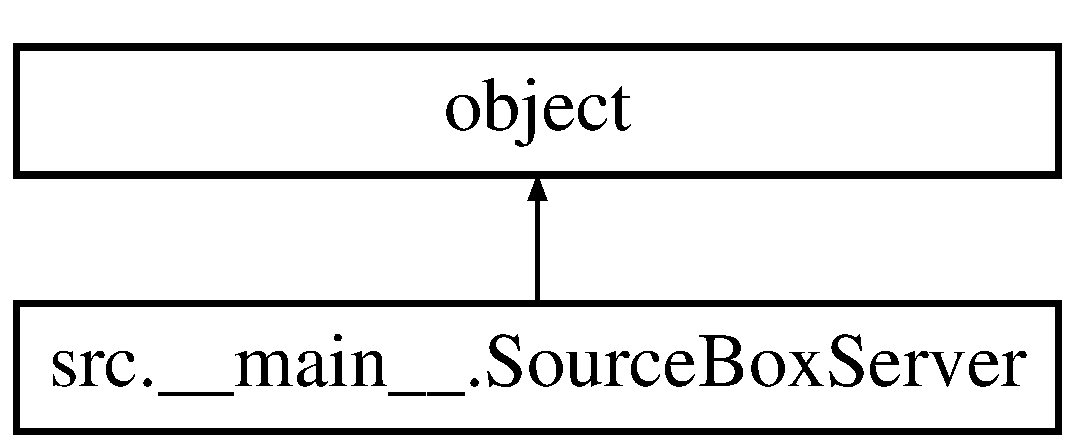
\includegraphics[height=2.000000cm]{classsrc_1_1____main_____1_1_source_box_server}
\end{center}
\end{figure}
\subsection*{Public Member Functions}
\begin{DoxyCompactItemize}
\item 
\hypertarget{classsrc_1_1____main_____1_1_source_box_server_ae7895f894241f906a0dc8378c76eb7e3}{def {\bfseries \-\_\-\-\_\-init\-\_\-\-\_\-}}\label{classsrc_1_1____main_____1_1_source_box_server_ae7895f894241f906a0dc8378c76eb7e3}

\item 
\hypertarget{classsrc_1_1____main_____1_1_source_box_server_a3cf42cc197094e86f618da7b17934c34}{def {\bfseries command\-\_\-loop}}\label{classsrc_1_1____main_____1_1_source_box_server_a3cf42cc197094e86f618da7b17934c34}

\end{DoxyCompactItemize}


The documentation for this class was generated from the following file\-:\begin{DoxyCompactItemize}
\item 
sourcebox-\/server/src/\-\_\-\-\_\-main\-\_\-\-\_\-.\-py\end{DoxyCompactItemize}

%--- End generated contents ---

% Index
\newpage
\phantomsection
\addcontentsline{toc}{part}{Index}
\printindex

\end{document}
